\chapter{Instructions for accessibility}


\section{What is the purpose of this document?}
%
According to the MARP (Manual of Academic Regulations and Procedures for Postgraduate Research), the formatting of PhD thesis must follow Lancaster University's guidance on accessible documents and resources (see Appendix 2, Point 8).
This document is a template you can use for your PhD thesis to fulfil this requirement, and also it gives you some useful advice and information.

Further this document is created using the relative new document tagging system. It is created so that it runs under pdflatex and under LuaLaTeX, and also under MikteX and TeXLive.
From an accessibility point of view, LuaLaTeX together with a recent TeX Live installation is the recommended way.
\begin{center}
\emph{However, it is important that  you are using the latest version of LaTeX}
\end{center}

This file was created on 30.5.2025 and updated on 22.2.2026 by Dirk Zeindler. If you have any comments, suggestions or corrections then please contact the disability officer.

\section{A note on using the template}

This template is designed so that you do not need to change much about your
usual way of writing \LaTeX{} documents.  Most of the accessibility features
(such as tagging, MathML, and structure) are handled automatically in the
background.  If you use the environments provided in this template in the
standard way, you will already produce a document that is much more accessible
than a normal \LaTeX{} PDF.  Only a few small rules need to be followed, which
are described in this chapter.


\section{What is accessibility?}
\label{sec:what-is-accessibility}
Document accessibility refers to how easily people, including those with disabilities, can perceive, understand, navigate, and interact with its content. Making a document accessible ensures that everyone, including those with visual, auditory, cognitive, or motor impairments, can access and use its information.
This is often important for legal purposes. For example, under the Equality Act of 2010, higher education providers have a duty to make reasonable adjustments that enable disabled students to access the full student learning experience.




\section{Why does the default LaTeX-to-PDF create inaccessible PDFs?}
%
\LaTeX{} was created in 1984 as a typesetting language for mathematical notation and for producing professional-looking documents suitable for printing. 
Requirements have changed since then. 
In particular, there is now also a need to produce accessible PDFs, which are readable by a screen reader.
%
The three main problems with the conversion from \LaTeX{} to PDF are that 
\begin{itemize}
	\item that equations cannot be read by screen readers,
	\item it is not possible to add alternative text to images and
	\item PDFs are not tagged, i.e. they do not contain tags 
	\footnote{Tags are embedded within the pdf and are invisible to the reader. Screen readers uses them to identify headings, paragraphs, lists, footnotes, images and tables. Also, tags are used to store additional information such as alternative text.}. 
\end{itemize}
Therefore, from August 2020, PDFs generated from \LaTeX{} using the default conversion to PDF should not be considered accessible.
The \LaTeX{} community is aware of this problem and is working hard to resolve these.
There has been very good process in the recent year, see for instance the
\href{https://latex3.github.io/tagging-project/}{\textcolor{blue}{LaTeX Tagging Project}}.
In particular, this document is using the new pdf tagging system, which produces pdfs that are very close to fulfill the accessibility standards. 

\section{Advice how to create (almost) accessible pdfs with \LaTeX}
\label{sec:advice-how-to-create-almost-accessible-documents-with-latex}

You can find on the site \href{https://portal.lancaster.ac.uk/ask/checklist-latex}{Accessibility checklist for LaTeX documents} some information of Lancaster University how to create accessible documents. 
You will see that most of the advice is either already implemented in this template or something you do anyway.
Here some additional advice.
\begin{itemize}
\item If you would like to emphasis some text than you should use \verb|\emph{}| instead of \verb|\textit{}|.
\item If you need to insert hyperlinks, the full web address can often be very long. In this situation, you can use the command \verb|\href{url}{linktext}| rather than \verb|\url|. 
You should avoid long raw URLs in text, and do not use `click here' as the link text.
Use a descriptive text instead, such as `More information can be found on ASK', to convey clear and accurate information about the destination.
\item For tables, it's important to use a header row, and if needed, a column header for structure and navigation. For tables that span across pages, make sure to repeat the header row at the top of each page.
\item People with visual impairments often cannot perceive images or diagrams clearly, which makes it difficult for them to understand their intended meaning.
Therefore, it is important to provide each image or diagram with a short descriptive text that can be read aloud by a screen reader, ensuring that the visual content remains accessible.
This description is called \emph{alternative text} (alt text).  
The tagging system provides a simple way to add alternative text
directly to \verb|\includegraphics|:
%
\begin{verbatim}
\begin{figure}
	\centering
	\includegraphics[alt={A placeholder image.}]{example-image}
	\caption{An example figure}
\end{figure}
\end{verbatim}
For guidance on how to write effective alternative text, useful tips can be found on the  
\href{https://portal.lancaster.ac.uk/ask/digital/accessibility/accessibility-guides/adding-alternative-text-to-diagrams-and-images/}
{\textcolor{blue}{Lancaster University page on adding alternative text}}.
You can find some examples in the Section~\ref{sec:figures}.
\end{itemize}

\subsection{Cross-references}

Cross-references are an essential part of an accessible document, as they help
screen readers and other assistive technologies navigate the content.  
You should always use the commands \verb|\label| and \verb|\ref| (or
\verb|\eqref| for equations) to refer to numbered objects such as figures,
tables, equations or theorems.  For example:

\begin{verbatim}
	As shown in Theorem~\ref{thm:main}, ...
	See Figure~\ref{fig:example}.
	From Table~\ref{tab:data} we observe that ...
\end{verbatim}

Never type reference numbers manually.. This is error‑prone, time‑consuming,
and breaks navigation for screen‑reader users.  
Using \verb|\label| and \verb|\ref| keeps all references up to date
automatically and makes the document easier to navigate in both print and
digital formats.

\subsection{Tips for accessible mathematics}

The new LaTeX tagging system automatically generates semantic MathML for
mathematical expressions, which greatly improves accessibility in the long
term.  To ensure correct results, consider the following guidelines:

\begin{itemize}
	\item Use standard \LaTeX{} math commands and environments, such as
	\verb|equation|, \verb|align|, or \verb|\[...\]|.
	\item Avoid manually inserting line breaks inside equations; instead, use
	\verb|align| or \verb|split|.
	\item Write inline mathematics sparingly and keep it short.
	\item Do not include long pieces of text inside math mode; screen readers
	cannot parse such content correctly.
	\item Avoid inserting mathematical expressions as images.  They cannot be
	read by assistive technologies.
\end{itemize}

At present, most screen readers cannot yet read MathML embedded in PDF files,
but this is expected to improve as PDF/UA--2 support evolves.

\subsection{Bibliography and citations}

The bibliography is automatically integrated into the document’s tag structure.
To ensure accessibility:

\begin{itemize}
	\item Use either \texttt{bibtex} or \texttt{biblatex}.  Both approaches
	generate structured bibliography entries.
	\item Do not type references manually; this produces untagged text.
	\item If you include URLs or DOIs, use \verb|\href| with descriptive link
	text rather than showing raw URLs.
\end{itemize}

A typical workflow is to maintain a \texttt{.bib} file and run
\texttt{bibtex} or \texttt{biber} to generate the bibliography.  This ensures
consistent formatting and correct tagging.

\subsection{Common pitfalls to avoid}

When creating an accessible document, the following common mistakes should be
avoided:

\begin{itemize}
	\item Do not use \verb|\textit| to emphasise text; use \verb|\emph| instead,
	as it conveys semantic emphasis.
	\item Do not use colour alone to convey meaning.  Always provide a textual
	description as well.
	\item Do not insert multiple spaces, \verb|\quad|, or manual positioning to
	adjust layout.  Use proper LaTeX environments instead.
	\item Avoid decorative images or diagrams unless you mark them as \verb|artifact| so
	that screen readers skip them.
	\item Avoid complex TikZ overlays or highly custom drawing code, as these are
	not yet fully supported by the tagging system.
	\item Do not manually format bibliographic entries.
	Always use a bibliography tool such as \texttt{bibtex} or
	\texttt{biblatex}.
	\item Avoid packages that are not compatible with the tagging system,
	such as \texttt{listings}, \texttt{minted} and some extended
	verbatim packages.
\end{itemize}

\section{Practical workflow for accessible compilation}
\label{sec:practical_advice}

The following recommendations address common issues that arise when working with the accessible template:

\begin{enumerate}
\item 
Enabling the command \verb|\DocumentMetadata| significantly reduces the compilation speed of a document. For larger documents, compilation may take up to several minutes.

It is therefore recommended to disable \verb|\DocumentMetadata| during development (for example by commenting it out) in order to speed up compilation and simplify debugging. For the final version of the document, \verb|\DocumentMetadata| should be re‑enabled to produce an accessible PDF.

It is advisable to enable \verb|\DocumentMetadata| occasionally during development to ensure that no compatibility or compilation issues arise.

\item
The compilation with \verb|\DocumentMetadata| is not yet fully as robust as for a standard \LaTeX{} document. In particular, compilation may occasionally fail even though there is no error in the source code. Furthermore, a failed compilation can corrupt the generated auxiliary files (e.g.\ \texttt{.aux}, \texttt{.toc}, \texttt{.out}, \texttt{.log}) and lead to additional, seemingly unrelated error messages.

If unexpected or unusual errors occur, it is therefore recommended to delete all auxiliary files and recompile the document from scratch. In particular, \verb|\DocumentMetadata| generates an auxiliary HTML file. This is not a usable HTML version of the document and should also be removed during cleanup.
\item
When switching between development mode and the accessible version (with \verb|\DocumentMetadata| enabled), a clean compilation is recommended, i.e. to delete all auxiliary files. 
This avoids inconsistencies and compilation errors.
\item
Not all \LaTeX{} packages are compatible with the PDF tagging system. 
If unexpected errors occur when \verb|\DocumentMetadata| is enabled, it is advisable to temporarily disable recently added packages in order to identify potential incompatibilities.

As a first indication, external resources (including AI tools) may help to assess whether a particular package is compatible with \verb|\DocumentMetadata|. 

This template already includes a set of commonly used packages that are known to work reliably with the tagging system. In many cases, no additional packages are needed, and it is advisable to only introduce new packages when necessary.
\item 
  The spacing in this template is slightly more structured than in a standard \LaTeX{} document. This improves readability and leads to a more compact and visually consistent layout.

    A disadvantage is that less vertical space is available for figures and tables. In particular, it may happen that \LaTeX{} is not able to place a figure or table. In such cases, you may receive a message such as \emph{Float(s) lost!}, and the figure or table may disappear from the output. In some situations, compilation may fail completely and no PDF is generated.
    This often occurs when using restrictive placement options such as \verb|[h]| or \verb|[h!]|, in particular inside structured environments like theorem environments.

    To avoid this issue, you can replace the floating environment with a non-floating construction. A standard floating figure is defined as:
\begin{verbatim}
\begin{figure}
  \centering
  \includegraphics[alt={A placeholder image.}]{example-image}
  \caption{An example figure}
  \label{fig:example_figure}
\end{figure}
\end{verbatim}
    This can be replaced by the following non-floating construction:
\begin{verbatim}
\begin{center}
  \includegraphics[alt={A placeholder image.}]{example-image}
  \captionof{figure}{An example figure}
  \label{fig:example_figure}
\end{center}
\end{verbatim}
This ensures that the figure appears exactly at the desired location and avoids issues with \LaTeX{}'s float placement mechanism.

The same approach can be used for tables by using \verb|\captionof{table}|.
\end{enumerate}

\section{Examples of some code}
\label{sec:exmaples_code}

In this section, we give some examples to illustrate how things look and how they can be implemented.

\subsection{Equations}
We have
\begin{align}
	B(M,N)
	=
	\sum_{m,n}\alpha_m\beta_n \exp\left(2\pi i \frac{\overline{m}}{n}\right)   
\end{align}

\subsection{Definitions, Theorems and more}
\label{sec:definitions-and-theorems}
%
The theorem environments in this document are implemented using the \verb|tcolorbox| package.
The setup in the preamble is somewhat involved, but this has already been done for you.
If you are happy with the appearance of the theorem boxes, you do not need to change anything — simply use the environments in the usual way, e.g.\ 
\begin{center}
\verb|\begin{theorem}...\end{theorem}|.
\end{center}
A classical solution without frames is also included in the preamble, but commented out.

%\endinput

\begin{definition}
	\label{def:countable set}
	A set $\Omega$ is \emph{countable}\index{countable} if one can assign to each $\omega\in\Omega$ a natural number $n\in\N$ so that each $n\in\N$ correspond to at most one $\omega\in\Omega$. 
	If this is not possible, we call the set \emph{uncountable}\index{uncountable}.
\end{definition}
%


\begin{example}
	\label{bsp:elementary_examples}
	The sets $\N$, $\Z$ and $\Q$ are countable.
	Furthermore any subset of  $\N$, $\Z$ and $\Q$ are countable.
	However, not each set is countable. For instance, $\R$ and $\C$ are not countable.
\end{example}


\begin{lemma}
	\label{lem:not_rep_measure}
	Consider an arbitrage free finite market model, realised on the probability space $(\Omega, \mathbb{P})$, and 
	let $\Phi$ be an $\mathcal{F}_T$ measurable random variable, which is not replicable.
	Then there exist \emph{risk neutral measures} $\mathbb{P}_*$ and $\mathbb{P}'_*$ such that
	%
	\begin{align}
		\mathbb{E}_*[\Phi]\neq \mathbb{E}'_*[\Phi].
	\end{align} 
\end{lemma}


\begin{theorem}[{First fundamental theorem of asset pricing, e.g. \cite[Thm~4.2.6]{Turner_Zeindler_2023}}]
	\label{thm:fund_thm1}
	A finite market model is arbitrage free if and only if there exists at least one \emph{risk neutral probability measure} $\mathbb{P}_*$.
\end{theorem}
%
\begin{corollary}
If a finite market model is arbitrage free  but not complete  then there exists infinitely many \emph{risk neutral probability measure} $\mathbb{P}_*$.
\end{corollary}

\subsection{Enumerates and itemize}

An example of a numbered list:
\begin{enumerate}
	\item The first case.
	\begin{enumerate}
		\item A subcase.
		\item Another subcase.
	\end{enumerate}	
	\item The second case.
	\item The third case.
\end{enumerate}

An example of a unnumbered list
\begin{itemize}
	\item The first case.
	\begin{itemize}
		\item A subcase.
		\item Another subcase.
	\end{itemize}	
	\item The second case.
	\item The third case.
\end{itemize}

\subsection{Figures}
\label{sec:figures}

Figure~\ref{fig:A_cup_B} contains an example of a Figure with alternative text.
\begin{figure}[ht]
	\centering
		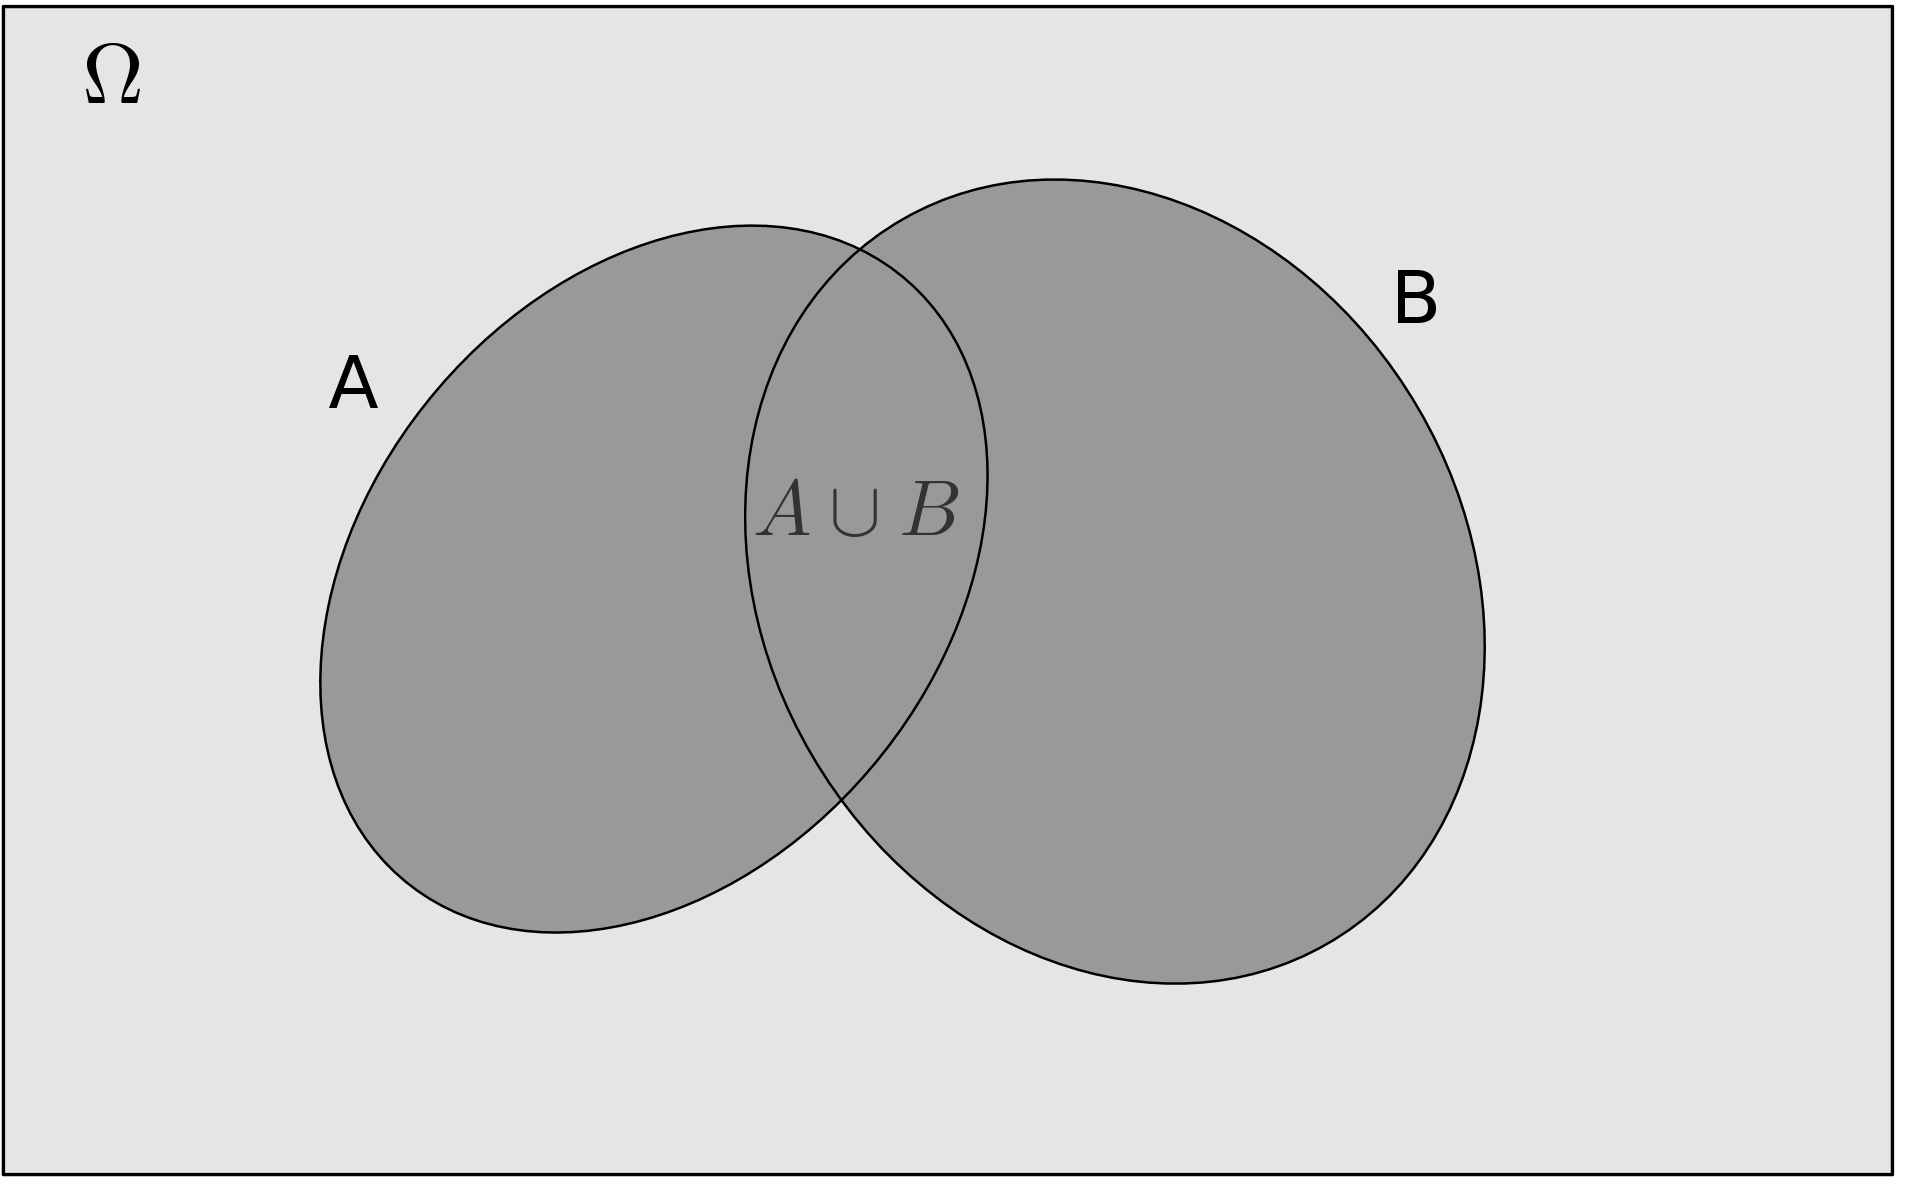
\includegraphics[width=0.5\textwidth, alt={Venn diagramm of the union of the sets A and B}]{images/grundmenge_union}	
	\caption{Illustration of $A\cup B$.}
	\label{fig:A_cup_B}
\end{figure}

Figure~\ref{fig:illust_venn_pb} is an example of a figure with subfigures and alternative text.
In particular, you can refer to the entire Figure~\ref{fig:illust_venn_pb} or to an individual subfigure such as Figure~\ref{fig:cup}.

Subfigures can be very useful, but they may further complicate the placement of figures and may interfere with the tagging when \verb|\DocumentMetadata| is enabled. Therefore, they should be used with care.
%
\begin{figure}[ht]
	\centering
	\begin{subfigure}[c]{0.48\textwidth}
		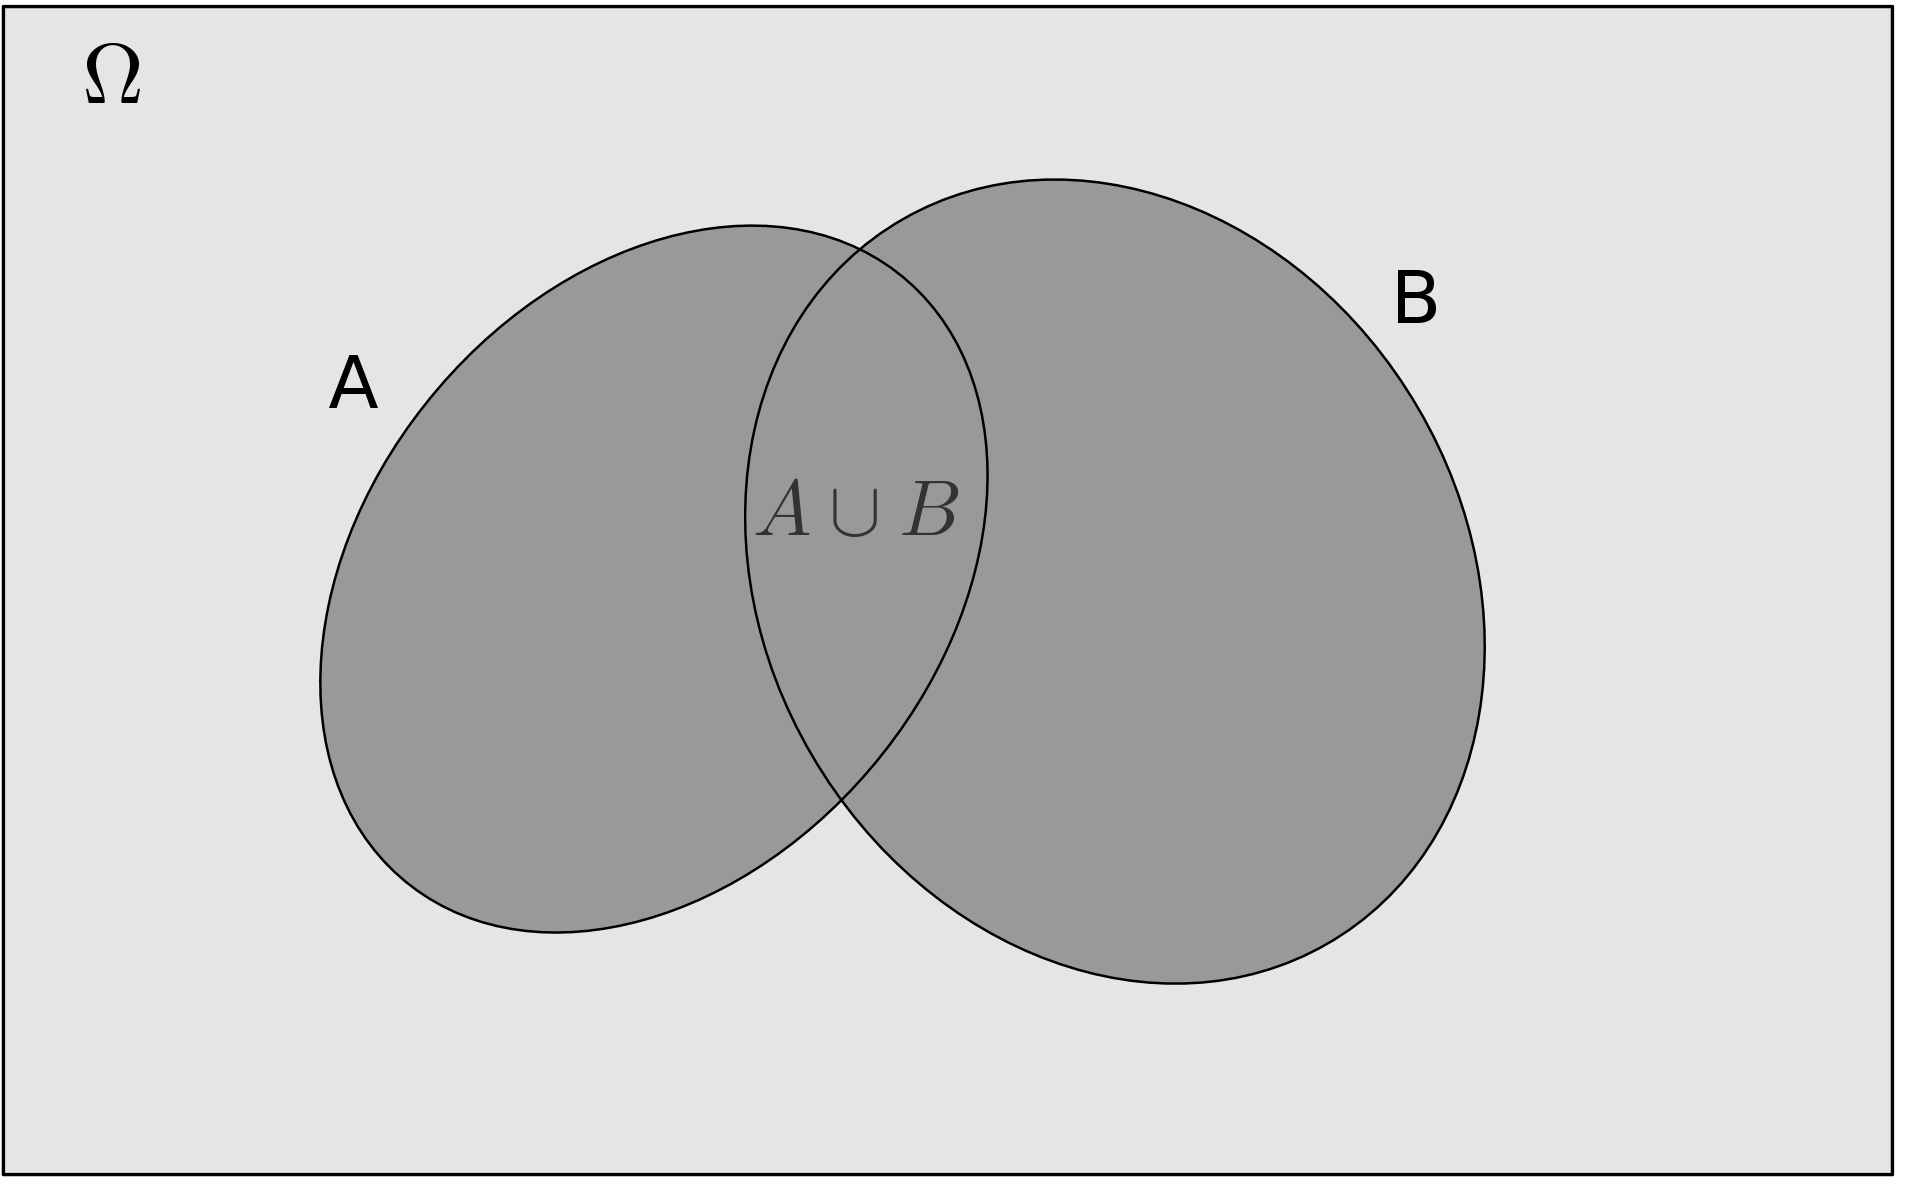
\includegraphics[width=1\textwidth, alt={Venn diagramm of the union of the sets A and B}]{images/grundmenge_union}	
		\caption{`$A$ or $B$', the union $A\cup B$}
		\label{fig:cup}
	\end{subfigure}
	%
	\begin{subfigure}[c]{0.48\textwidth}
		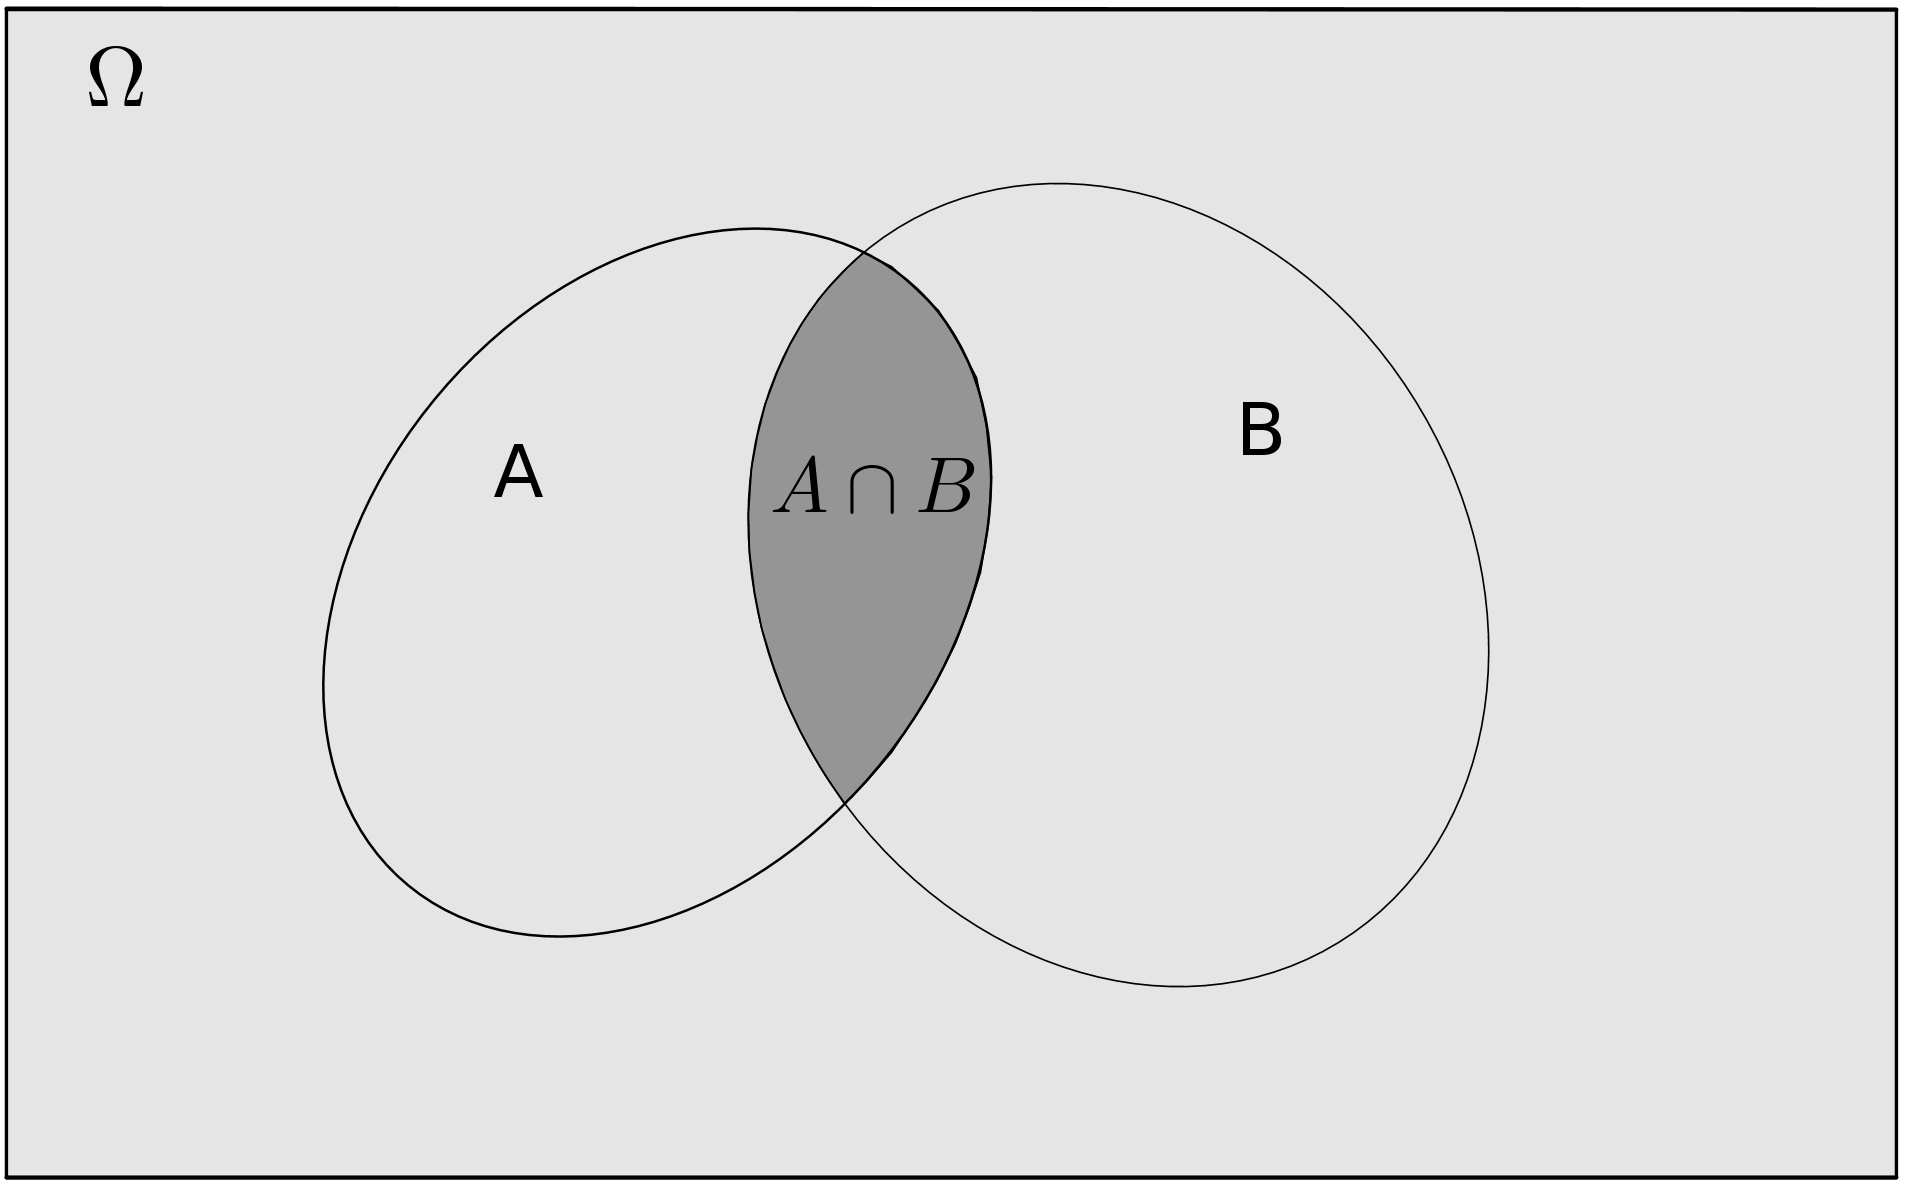
\includegraphics[width=1\textwidth, alt={Venn diagramm of the intersection of the sets A and B}]{images/grundmenge_intersection}
		\caption{`$A$ and $B$', the intersection $A\cap B$}
	\end{subfigure}
	\begin{subfigure}[c]{0.48\textwidth}
		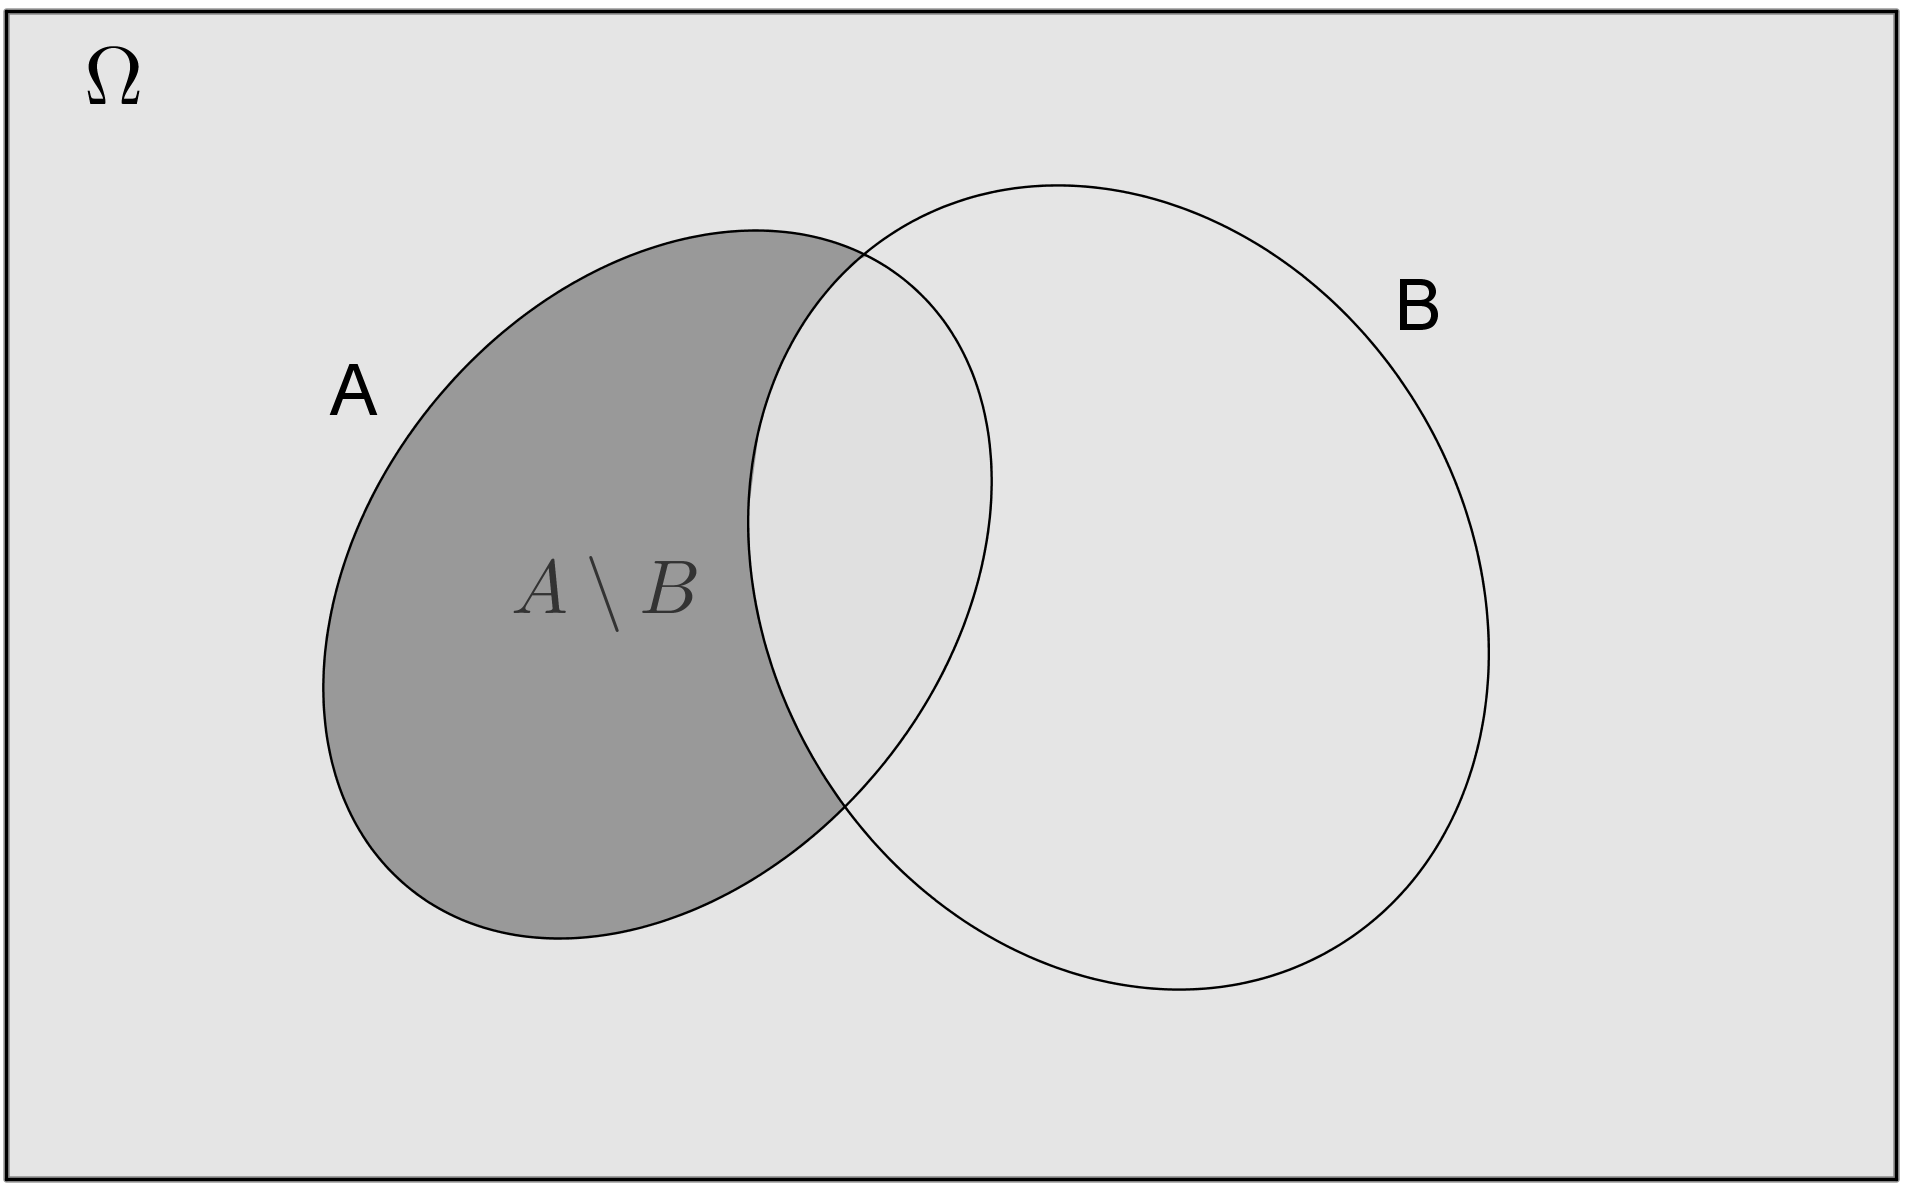
\includegraphics[width=1\textwidth, alt={Venn diagramm of the set difference of the sets A and B}]{images/grundmenge_setdiff}
		\caption{`$A$ but not $B$', the set difference $A\setminus B$}
	\end{subfigure}
	%
	\begin{subfigure}[c]{0.48\textwidth}
		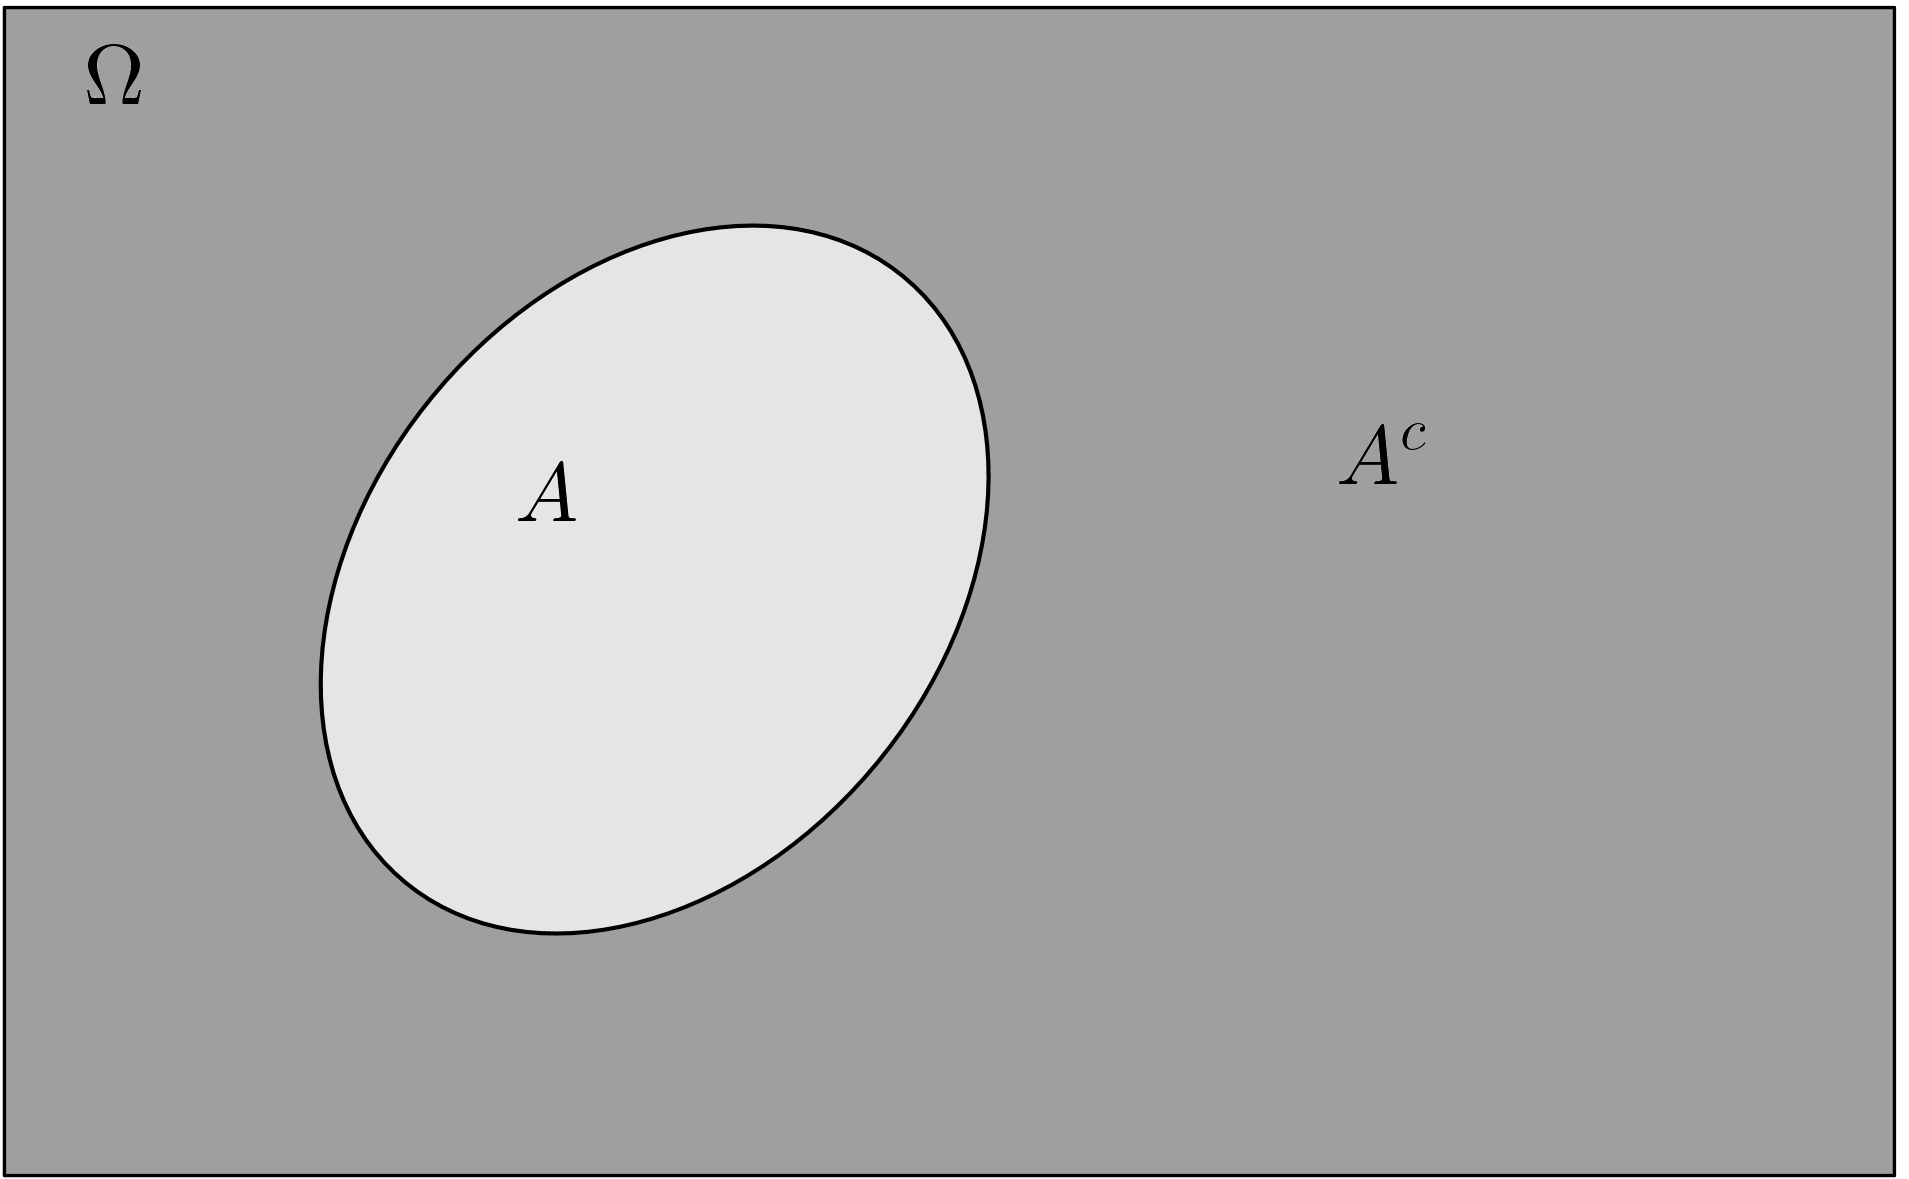
\includegraphics[width=1\textwidth, alt={Venn diagramm of the complement of the set A}]{images/grundmenge_complement3}
		\caption{`$A$ does not occur', the complement $A^c$}
	\end{subfigure}	
	%
	\caption{Illustration of $A\cup B$, $A\cap B$, $A\setminus B$, $A^c$.}
	\label{fig:illust_venn_pb}
\end{figure}

\newpage

\subsection{Tables}

The new tagging system also supports accessible tables.  In order for assistive
technologies to interpret a table correctly, it is important that the structure
is clear and that header cells are identified.  This template enables table
header rows globally through the option \verb|table/header-rows=1| inside the
\verb|\DocumentMetadata| declaration.

A simple example is shown below:

\begin{table}[ht]
	\centering
	\begin{tabular}{l r r}
		\hline
		\textbf{Item} & \textbf{Value A} & \textbf{Value B} \\
		\hline
		Apples  & 10 & 20 \\
		Bananas & 15 & 25 \\
		Cherries & 12 & 22 \\
		\hline
	\end{tabular}
	\caption{An example of an accessible table}
	\label{tab:example}
\end{table}

You can refer to this table using, for example, Table~\ref{tab:example}.
Ensure that the first row contains the header cells for assistive technologies.
If a table spans multiple pages, consider using the \texttt{longtable}
environment, which is partially supported.

\subsection{Program code}

Including program code in a thesis can be done in various ways, but the options
are limited when producing a tagged PDF/UA--2 document.

The classical \texttt{listings} package is widely used, but it is currently not
compatible with the new PDF tagging system and typically results in compilation
errors.  
Likewise, the popular \texttt{minted} package produces visually attractive,
colour-highlighted code, but it breaks the tagging structure when tagging is
enabled, even though the document may still compile successfully.

At present, there is unfortunately no reliable method to create a code
environment that is fully compatible with the tagging system and at the same
time provides a caption, numbering, and cross-referencing.  Properly tagged
verbatim content is still being developed within the Tagged PDF project.

For this reason, this template provides a simple code environment based on
\texttt{tcolorbox} and the standard \texttt{verbatim} environment.  This
approach is stable, preserves line breaks, and works reliably with tagged PDF
output.  For example:

\begin{codebox}
	\begin{verbatim}
		for i in range(10):
		print(i)
	\end{verbatim}
\end{codebox}

If you prefer not to use a frame around the code, you may simply use the 
\texttt{verbatim} environment on its own.


\section{Create accessible documents beyond pdf}
\label{sec:advice-how-to-create-accessible-documents}

You can ignore this section when creating your thesis.
However, for the sake of completeness, it's important to note that the difficulty of creating accessible documents isn't limited to LaTeX documents. This issue also applies to Word documents, scanned PDFs, and other documents.

You can find some information on the site \href{https://portal.lancaster.ac.uk/ask/digital/accessibility/accessibility-guides/creating-accessible-pdfs/}{Creating accessible PDFs} how to create accessible pdf's with Acrobat Pro.
Lancaster University has also created a Moodle course that covers
\href{https://development.lancaster.ac.uk/mod/page/view.php?id=446}{\textcolor{blue}{Creating Accessible Resources}} with Word, as well as how to make scanned PDFs accessible.



